% Lecture 2: Virtue Ethics and Modern Technology
% IT Ethics Course
% Brendan Shea, PhD - Rochester Community and Technical College

\documentclass[aspectratio=169]{beamer}

% Theme and styling
\usetheme{Madrid}
\usecolortheme{default}
\setbeamertemplate{navigation symbols}{}
\setbeamertemplate{footline}[frame number]

% Packages
\usepackage{tikz}
\usetikzlibrary{shapes,arrows,positioning,calc,fit,backgrounds}
\usepackage{booktabs}
\usepackage{array}
\usepackage{graphicx}

% Custom icons (text-based alternatives)
\newcommand{\faQuoteLeft}{\textbf{``}}
\newcommand{\faBalanceScale}{$\triangleright$}
\newcommand{\faComments}{\textbf{?}}
\newcommand{\faLightbulb}{$\star$}
\newcommand{\faThumbsUp}{\textbf{+}}
\newcommand{\faThumbsDown}{\textbf{--}}

% Custom colors
\definecolor{primaryblue}{RGB}{0,73,135}
\definecolor{accentgold}{RGB}{198,146,20}
\definecolor{darkgray}{RGB}{64,64,64}
\definecolor{lightgray}{RGB}{240,240,240}
\definecolor{quotegreen}{RGB}{34,139,34}

% Set theme colors
\setbeamercolor{structure}{fg=primaryblue}
\setbeamercolor{title}{fg=white,bg=primaryblue}
\setbeamercolor{frametitle}{fg=white,bg=primaryblue}
\setbeamercolor{block title}{fg=white,bg=primaryblue}
\setbeamercolor{block body}{bg=lightgray}
\setbeamercolor{block title alerted}{fg=white,bg=red!70!black}
\setbeamercolor{block body alerted}{bg=red!10}
\setbeamercolor{block title example}{fg=white,bg=quotegreen}
\setbeamercolor{block body example}{bg=green!5}

% Custom environments for consistent formatting

% Argument environment
\newenvironment{argument}{%
  \begin{block}{\faBalanceScale\hspace{0.5em}Argument in Standard Form}
  \begin{enumerate}
}{%
  \end{enumerate}
  \end{block}
}

% Discussion question environment
\newcommand{\discussion}[1]{%
  \begin{alertblock}{\faComments\hspace{0.5em}Discussion Question}
  #1
  \end{alertblock}
}

% Title information
\title[Virtue Ethics \& Technology]{Lecture 2: Virtue Ethics and Modern Technology}
\subtitle{Are Social Media and AI Making Us Stupider, Meaner, and Less Happy?}
\author{Brendan Shea, PhD}
\institute{Rochester Community and Technical College}
\date{}

\begin{document}

% ====================
% TITLE SLIDE
% ====================
\begin{frame}
\titlepage
\end{frame}

% ====================
% INTRODUCTION (Slides 2-4)
% ====================

\begin{frame}{The Big Question}
\begin{center}
\Large\textbf{Does technology shape who we become?}
\end{center}

\vspace{0.5em}
\begin{block}{Three Concerns About Modern Technology}
\begin{itemize}
  \item \textbf{Stupider?} Shortened attention spans, misinformation, ``structural stupidity''
  \item \textbf{Meaner?} Online trolling, polarization, loss of empathy
  \item \textbf{Less Happy?} Anxiety, depression, loneliness---especially among teens
\end{itemize}
\end{block}

\vspace{0.3em}
\begin{exampleblock}{The Virtue Ethics Approach}
Rather than asking ``Is this action right or wrong?'' we ask: \textbf{What kind of person am I becoming?}
\end{exampleblock}

\vspace{0.3em}
\discussion{Do you think you're a different person online than in person? Better or worse?}
\end{frame}

\begin{frame}{Why Virtue Ethics?}
\begin{columns}
\begin{column}{0.48\textwidth}
\begin{block}{Other Ethical Approaches}
\begin{itemize}
  \item \textbf{Consequentialism}: Focus on outcomes
  \item \textbf{Deontology}: Focus on rules and duties
  \item \textbf{Rights-based}: Focus on individual rights
\end{itemize}
\end{block}
\end{column}

\begin{column}{0.48\textwidth}
\begin{exampleblock}{Virtue Ethics}
\begin{itemize}
  \item Focus on \textbf{character formation}
  \item We become what we \textbf{repeatedly do}
  \item Technology shapes our \textbf{habits}
  \item Habits shape who we \textbf{are}
\end{itemize}
\end{exampleblock}
\end{column}
\end{columns}

\vspace{0.5em}
\begin{alertblock}{Key Insight}
If technology changes what we \textit{repeatedly do}, it changes \textit{who we become}.
\end{alertblock}
\end{frame}

\begin{frame}{Roadmap for Today}
\begin{center}
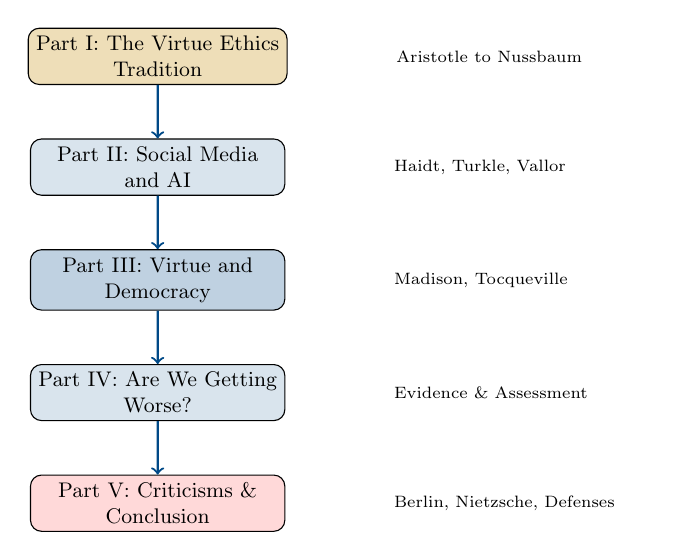
\begin{tikzpicture}[scale=0.85, transform shape,
    node distance=0.8cm,
    box/.style={draw, rounded corners, fill=primaryblue!15, minimum width=3.8cm, minimum height=0.8cm, align=center, font=\small}]
  
  \node[box, fill=accentgold!30] (part1) {Part I: The Virtue Ethics\\Tradition};
  \node[box, below=of part1] (part2) {Part II: Social Media\\and AI};
  \node[box, below=of part2, fill=primaryblue!25] (part3) {Part III: Virtue and\\Democracy };
  \node[box, below=of part3] (part4) {Part IV: Are We Getting\\Worse? };
  \node[box, below=of part4, fill=red!15] (part5) {Part V: Criticisms \&\\Conclusion };
  
  \draw[->, thick, primaryblue] (part1) -- (part2);
  \draw[->, thick, primaryblue] (part2) -- (part3);
  \draw[->, thick, primaryblue] (part3) -- (part4);
  \draw[->, thick, primaryblue] (part4) -- (part5);
  
  \node[right=1.5cm of part1, font=\scriptsize, text width=4cm] {Aristotle to Nussbaum};
  \node[right=1.5cm of part2, font=\scriptsize, text width=4cm] {Haidt, Turkle, Vallor};
  \node[right=1.5cm of part3, font=\scriptsize, text width=4cm] {Madison, Tocqueville};
  \node[right=1.5cm of part4, font=\scriptsize, text width=4cm] {Evidence \& Assessment};
  \node[right=1.5cm of part5, font=\scriptsize, text width=4cm] {Berlin, Nietzsche, Defenses};
\end{tikzpicture}
\end{center}
\end{frame}

% ====================
% PART I: THE VIRTUE ETHICS TRADITION (Slides 5-15)
% ====================

\begin{frame}{What Is a Virtue?}
\begin{block}{Definition}
A \textbf{virtue} is an \textit{excellent character trait}---a stable disposition to act, feel, and think in ways that promote human flourishing.
\end{block}

\vspace{0.3em}
\begin{columns}
\begin{column}{0.48\textwidth}
\begin{exampleblock}{Examples of Virtues}
\begin{itemize}
  \item \textbf{Courage}: Acting well despite fear
  \item \textbf{Temperance}: Moderation in pleasure
  \item \textbf{Honesty}: Truthfulness in word and deed
  \item \textbf{Justice}: Giving others their due
  \item \textbf{Wisdom}: Good practical judgment
\end{itemize}
\end{exampleblock}
\end{column}

\begin{column}{0.48\textwidth}
\begin{alertblock}{Examples of Vices}
\begin{itemize}
  \item \textbf{Cowardice}: Excessive fear
  \item \textbf{Intemperance}: Excess in pleasure
  \item \textbf{Dishonesty}: Deception
  \item \textbf{Injustice}: Taking more than one's share
  \item \textbf{Foolishness}: Poor judgment
\end{itemize}
\end{alertblock}
\end{column}
\end{columns}

\vspace{0.3em}
\discussion{Which virtues do you think are most important for life in the digital age?}
\end{frame}

\begin{frame}{Who Was Aristotle?}
\begin{columns}
\begin{column}{0.6\textwidth}
\begin{block}{Aristotle (384--322 BCE)}
\begin{itemize}
  \item Student of Plato, tutor to Alexander the Great
  \item Founded the Lyceum in Athens
  \item Wrote on logic, physics, biology, ethics, politics, poetry
  \item \textbf{\textit{Nicomachean Ethics}}: Most influential work on virtue
  \item Asked: ``What is the good life for a human being?''
\end{itemize}
\end{block}

\begin{exampleblock}{Why Aristotle Still Matters}
His framework for thinking about character, habit, and human flourishing remains remarkably relevant 2,400 years later.
\end{exampleblock}
\end{column}

\begin{column}{0.38\textwidth}
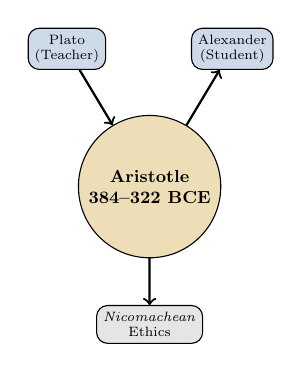
\begin{tikzpicture}[scale=0.7, transform shape]
  \node[draw, circle, fill=accentgold!30, minimum size=2cm, font=\small\bfseries, align=center] (aristotle) at (0,0) {Aristotle\\384--322 BCE};
  \node[draw, rounded corners, fill=primaryblue!20, font=\scriptsize, align=center] (plato) at (-1.5,2.5) {Plato\\(Teacher)};
  \node[draw, rounded corners, fill=primaryblue!20, font=\scriptsize, align=center] (alex) at (1.5,2.5) {Alexander\\(Student)};
  \node[draw, rounded corners, fill=gray!20, font=\scriptsize, align=center] (ethics) at (0,-2.5) {\textit{Nicomachean}\\Ethics};
  \draw[->, thick] (plato) -- (aristotle);
  \draw[->, thick] (aristotle) -- (alex);
  \draw[->, thick] (aristotle) -- (ethics);
\end{tikzpicture}
\end{column}
\end{columns}
\end{frame}

\begin{frame}{Aristotle's Key Ideas}
\begin{block}{Eudaimonia: Human Flourishing}
The goal of life is not just pleasure or wealth, but \textbf{eudaimonia}---living well and doing well, fulfilling our potential as human beings.
\end{block}

\vspace{0.3em}
\begin{exampleblock}{The Function Argument}
Just as a good knife cuts well (fulfills its function), a good \textit{human} lives according to \textbf{reason}---our distinctive capacity.
\end{exampleblock}

\vspace{0.3em}
\begin{alertblock}{Virtue as Habit}
``We become just by doing just acts, temperate by doing temperate acts, brave by doing brave acts.'' --- Aristotle, \textit{Nicomachean Ethics} II.1
\end{alertblock}

\vspace{0.3em}
\begin{block}{\faLightbulb\hspace{0.3em}Implication for Technology}
If we become what we repeatedly do, then what we repeatedly do \textit{online} shapes our character.
\end{block}
\end{frame}

\begin{frame}{Aristotle's Virtues: The Doctrine of the Mean}
\begin{block}{The Golden Mean}
Virtue is a \textbf{mean} (middle point) between two vices: one of \textit{excess} and one of \textit{deficiency}.
\end{block}

\vspace{0.3em}
\begin{table}
\centering
\small
\begin{tabular}{@{}lccc@{}}
\toprule
\textbf{Sphere of Action} & \textbf{Deficiency (Vice)} & \textbf{Mean (Virtue)} & \textbf{Excess (Vice)} \\
\midrule
Fear and confidence & Cowardice & \textbf{Courage} & Recklessness \\
Pleasure and pain & Insensibility & \textbf{Temperance} & Self-indulgence \\
Giving money & Stinginess & \textbf{Generosity} & Prodigality \\
Self-regard & Self-deprecation & \textbf{Proper pride} & Vanity \\
Social interaction & Boorishness & \textbf{Wit} & Buffoonery \\
Truth about self & Self-deprecation & \textbf{Honesty} & Boastfulness \\
\bottomrule
\end{tabular}
\end{table}

\vspace{0.3em}
\discussion{Where would ``posting on social media'' fit? What's the virtuous mean between over-sharing and never engaging?}
\end{frame}

\begin{frame}{Phronesis: Practical Wisdom}
\begin{block}{Definition}
\textbf{Phronesis} (practical wisdom) is the master virtue---the ability to discern the right thing to do in particular circumstances.
\end{block}

\vspace{0.3em}
\begin{columns}
\begin{column}{0.48\textwidth}
\begin{exampleblock}{What Phronesis Requires}
\begin{itemize}
  \item Experience and good judgment
  \item Understanding context
  \item Balancing competing goods
  \item Knowing \textit{when}, \textit{how}, and \textit{to whom}
\end{itemize}
\end{exampleblock}
\end{column}

\begin{column}{0.48\textwidth}
\begin{alertblock}{Why It Matters for Tech}
\begin{itemize}
  \item Rules alone aren't enough
  \item Context changes everything
  \item Algorithms can't replace judgment
  \item We need wisdom, not just information
\end{itemize}
\end{alertblock}
\end{column}
\end{columns}

\vspace{0.3em}
\discussion{Can practical wisdom be taught? Can it be coded into an algorithm?}
\end{frame}

\begin{frame}{The Stoics: Epictetus on What We Control}
\begin{columns}
\begin{column}{0.6\textwidth}
\begin{block}{Epictetus (50--135 CE)}
\begin{itemize}
  \item Born a slave in Roman Empire
  \item Later freed, became influential philosopher
  \item Taught that virtue is the \textit{only} true good
  \item Key distinction: what's \textbf{up to us} vs. what's \textbf{not up to us}
\end{itemize}
\end{block}

\begin{exampleblock}{\faQuoteLeft\hspace{0.3em}Epictetus, \textit{Enchiridion}, Ch. 1}
\small
\textit{``Some things are within our power, while others are not. Within our power are opinion, motivation, desire, aversion... Not within our power are our body, our property, reputation, office...''}
\end{exampleblock}
\end{column}

\begin{column}{0.38\textwidth}
\begin{alertblock}{Applied to Social Media}
\begin{itemize}
  \item \textbf{Up to us}: How we respond, what we post, whether we engage
  \item \textbf{Not up to us}: Others' reactions, likes, viral spread, algorithmic promotion
\end{itemize}
\end{alertblock}
\end{column}
\end{columns}
\end{frame}

\begin{frame}{Aquinas: Virtue Meets Christianity}
\begin{block}{Thomas Aquinas (1225--1274)}
\begin{itemize}
  \item Dominican friar, synthesized Aristotle with Christian theology
  \item Adopted Aristotle's \textbf{cardinal virtues}: prudence, justice, fortitude, temperance
  \item Added the \textbf{theological virtues}: faith, hope, and love (charity)
\end{itemize}
\end{block}

\vspace{0.3em}
\begin{columns}
\begin{column}{0.48\textwidth}
\begin{exampleblock}{Cardinal Virtues}
\begin{itemize}
  \item Acquired through \textbf{practice}
  \item Accessible to all humans
  \item Based on \textbf{reason}
\end{itemize}
\end{exampleblock}
\end{column}

\begin{column}{0.48\textwidth}
\begin{block}{Theological Virtues}
\begin{itemize}
  \item Infused by \textbf{divine grace}
  \item Orient us toward God
  \item Perfect the natural virtues
\end{itemize}
\end{block}
\end{column}
\end{columns}

\vspace{0.3em}
\begin{alertblock}{Key Contribution}
Aquinas emphasized that virtues must be integrated---you can't be truly just without also being wise, temperate, and courageous.
\end{alertblock}
\end{frame}

\begin{frame}{John Dewey: Virtue in Democracy}
\begin{block}{John Dewey (1859--1952)}
\begin{itemize}
  \small
  \item American pragmatist philosopher
  \item Emphasized \textbf{democratic virtues}: open-mindedness, intellectual humility, cooperative inquiry
  \item Education as character formation for democratic citizenship
  \item Influenced progressive education movement
\end{itemize}
\end{block}

\vspace{0.3em}
\begin{exampleblock}{Dewey's Democratic Virtues}
\begin{itemize}
  \small
  \item \textbf{Open-mindedness}: Willingness to consider new evidence and perspectives
  \item \textbf{Intellectual humility}: Recognizing the limits of one's knowledge
  \item \textbf{Cooperative inquiry}: Working with others to solve problems
  \item \textbf{Experimental attitude}: Treating beliefs as hypotheses to be tested
\end{itemize}
\end{exampleblock}

\vspace{0.3em}
\small
\discussion{Does social media encourage or discourage Dewey's democratic virtues?}
\end{frame}

\begin{frame}{Martha Nussbaum: Capabilities and Flourishing}
\begin{columns}
\begin{column}{0.58\textwidth}
\begin{block}{Martha Nussbaum (b. 1947)}
\begin{itemize}
  \item Contemporary philosopher at University of Chicago
  \item Developed the \textbf{capabilities approach} to human development
  \item Key works: \textit{The Fragility of Goodness}, \textit{Not for Profit}, \textit{Political Emotions}
  \item Argues emotions are \textbf{intelligent responses} that matter for ethics
\end{itemize}
\end{block}

\begin{exampleblock}{The Capabilities Approach}
Justice requires ensuring people have the \textbf{capability} to achieve various ``functionings''---being healthy, educated, politically active, etc.
\end{exampleblock}
\end{column}

\begin{column}{0.4\textwidth}
\begin{alertblock}{Central Human Capabilities}
\footnotesize
\begin{enumerate}
  \item Life
  \item Bodily health
  \item Bodily integrity
  \item Senses, imagination, thought
  \item Emotions
  \item Practical reason
  \item Affiliation
  \item Other species
  \item Play
  \item Control over environment
\end{enumerate}
\end{alertblock}
\end{column}
\end{columns}
\end{frame}

\begin{frame}{Virtue Beyond the West}
\begin{table}
\centering
\small
\begin{tabular}{@{}p{2.5cm}p{4cm}p{6cm}@{}}
\toprule
\textbf{Tradition} & \textbf{Key Virtues} & \textbf{Central Idea} \\
\midrule
\textbf{Confucianism} & \textit{Ren} (benevolence), \textit{Li} (ritual propriety), \textit{Yi} (righteousness) & Virtue cultivated through proper relationships and social roles \\
\addlinespace
\textbf{Buddhism} & Compassion, mindfulness, equanimity, non-attachment & Virtue as liberation from suffering through wisdom \\
\addlinespace
\textbf{Ubuntu} (African) & Humaneness, community, interdependence & ``I am because we are''---virtue is inherently relational \\
\addlinespace
\textbf{Aristotelian} & Courage, temperance, justice, wisdom & Virtue as excellence of character enabling flourishing \\
\bottomrule
\end{tabular}
\end{table}

\vspace{0.5em}
\begin{exampleblock}{Common Threads}
Despite differences, these traditions share: emphasis on \textbf{character formation}, \textbf{community}, \textbf{practice}, and the idea that virtue must be \textbf{cultivated} over time.
\end{exampleblock}
\end{frame}

\begin{frame}{What Unites Virtue Ethicists?}
\begin{center}
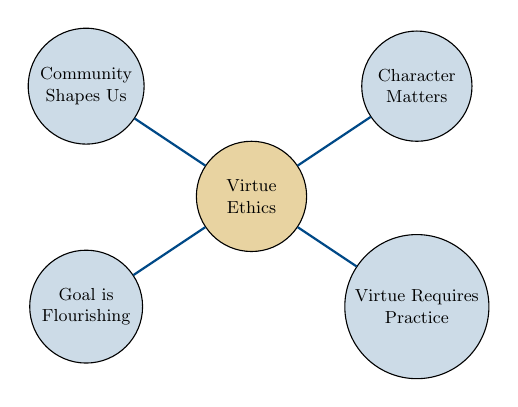
\begin{tikzpicture}[scale=0.7, transform shape,
    concept/.style={draw, circle, fill=primaryblue!20, minimum size=2cm, align=center, font=\small}]
  
  \node[concept, fill=accentgold!40] (center) at (0,0) {Virtue\\Ethics};
  \node[concept] (character) at (3,2) {Character\\Matters};
  \node[concept] (practice) at (3,-2) {Virtue Requires\\Practice};
  \node[concept] (community) at (-3,2) {Community\\Shapes Us};
  \node[concept] (flourishing) at (-3,-2) {Goal is\\Flourishing};
  
  \draw[thick, primaryblue] (center) -- (character);
  \draw[thick, primaryblue] (center) -- (practice);
  \draw[thick, primaryblue] (center) -- (community);
  \draw[thick, primaryblue] (center) -- (flourishing);
\end{tikzpicture}
\end{center}

\vspace{0.3em}
\begin{block}{Summary: The Virtue Ethics Framework}
\begin{itemize}
  \small
  \item Ethics is about \textbf{who we are}, not just what we do
  \item Virtue is developed through \textbf{habituation and practice}
  \item We need \textbf{practical wisdom} to navigate particular situations
  \item The goal is \textbf{eudaimonia}---a flourishing human life
\end{itemize}
\end{block}
\end{frame}

% ====================
% PART II: SOCIAL MEDIA AND AI (Slides 16-25)
% ====================

\begin{frame}{A Brief History of Social Media}
\begin{center}
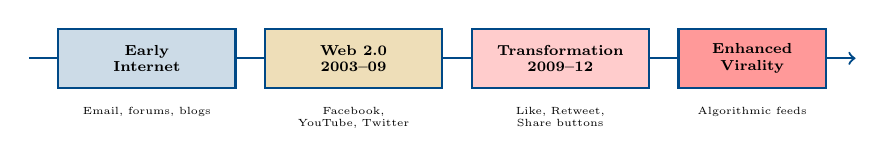
\begin{tikzpicture}[scale=0.75, transform shape]
  \draw[thick, ->, primaryblue] (0,0) -- (14,0);
  
  % Era markers
  \draw[thick, primaryblue, fill=primaryblue!20] (0.5,-0.5) rectangle (3.5,0.5);
  \draw[thick, primaryblue, fill=accentgold!30] (4,-0.5) rectangle (7,0.5);
  \draw[thick, primaryblue, fill=red!20] (7.5,-0.5) rectangle (10.5,0.5);
  \draw[thick, primaryblue, fill=red!40] (11,-0.5) rectangle (13.5,0.5);
  
  \node[font=\scriptsize\bfseries, align=center] at (2,0) {Early\\Internet};
  \node[font=\scriptsize\bfseries, align=center] at (5.5,0) {Web 2.0\\2003--09};
  \node[font=\scriptsize\bfseries, align=center] at (9,0) {Transformation\\2009--12};
  \node[font=\scriptsize\bfseries, align=center] at (12.25,0) {Enhanced\\Virality};
  
  % Key events
  \node[below, font=\tiny, text width=2.5cm, align=center] at (2,-0.7) {Email, forums, blogs};
  \node[below, font=\tiny, text width=2.5cm, align=center] at (5.5,-0.7) {Facebook, YouTube, Twitter};
  \node[below, font=\tiny, text width=2.5cm, align=center] at (9,-0.7) {Like, Retweet, Share buttons};
  \node[below, font=\tiny, text width=2.5cm, align=center] at (12.25,-0.7) {Algorithmic feeds};
\end{tikzpicture}
\end{center}

\vspace{0.5em}
\begin{alertblock}{The Key Transformation (2009--2012)}
Social media shifted from \textbf{connecting friends} to \textbf{maximizing engagement}. The introduction of the Like button (2009), Retweet (2009), and algorithmic feeds changed everything.
\end{alertblock}

\vspace{0.3em}
\discussion{Do you remember social media before algorithmic feeds? What was different?}
\end{frame}

\begin{frame}{The Virality Machine}
\begin{columns}
\begin{column}{0.5\textwidth}
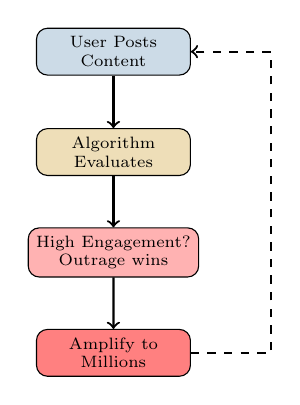
\begin{tikzpicture}[scale=0.85, transform shape,
    box/.style={draw, rounded corners, minimum width=2.3cm, minimum height=0.7cm, align=center, font=\scriptsize}]
  
  \node[box, fill=primaryblue!20] (user) at (0,2.5) {User Posts\\Content};
  \node[box, fill=accentgold!30] (algo) at (0,1) {Algorithm\\Evaluates};
  \node[box, fill=red!30] (engage) at (0,-0.5) {High Engagement?\\Outrage wins};
  \node[box, fill=red!50] (amplify) at (0,-2) {Amplify to\\Millions};
  
  \draw[->, thick] (user) -- (algo);
  \draw[->, thick] (algo) -- (engage);
  \draw[->, thick] (engage) -- (amplify);
  \draw[->, thick, dashed] (amplify.east) -- ++(1.2,0) |- (user.east);
\end{tikzpicture}
\end{column}

\begin{column}{0.48\textwidth}
\begin{block}{What Algorithms Optimize}
\footnotesize
Engagement, clicks, shares---\textbf{not} truth, wisdom, or flourishing
\end{block}

\begin{alertblock}{The Problem}
\footnotesize
Platforms are designed to capture attention. Outrage is more engaging than nuance.
\end{alertblock}
\end{column}
\end{columns}

\vspace{0.3em}
\begin{exampleblock}{\faLightbulb\hspace{0.3em}Key Insight}
\small
The platforms are designed to capture attention, not to make us better people.
\end{exampleblock}
\end{frame}

\begin{frame}{Quote: Jonathan Haidt on Babel}
\begin{exampleblock}{\faQuoteLeft\hspace{0.5em}Jonathan Haidt, ``Why the Past 10 Years of American Life Have Been Uniquely Stupid'' (2022)}
\small
\textit{``The story of Babel is the best metaphor I have found for what happened to America in the 2010s... \textbf{Something went terribly wrong}, very suddenly. We are disoriented, unable to speak the same language or recognize the same truth.''}

\vspace{0.3em}
\textit{``Social media has both \textbf{magnified and weaponized} the frivolous. Is it any wonder, then, that the public square has become so dull, so crude, so dominated by posturing and so hostile to genuine dialogue?''}
\end{exampleblock}

\vspace{0.3em}
\begin{block}{\faLightbulb\hspace{0.3em}The Babel Metaphor}
Like the Tower of Babel, we've lost our common language---our ability to share a reality.
\end{block}
\end{frame}

\begin{frame}{Hubert Dreyfus: The Risk of Disembodiment}
\begin{block}{Hubert Dreyfus (1929--2017)}
\begin{itemize}
  \item Philosopher at UC Berkeley, early critic of AI
  \item Argued that human intelligence is fundamentally \textbf{embodied}
  \item \textit{On the Internet} (2001): Warned about online disembodiment
\end{itemize}
\end{block}

\vspace{0.3em}
\begin{columns}
\begin{column}{0.48\textwidth}
\begin{exampleblock}{Embodied Commitment}
Real-world actions involve \textbf{risk}---our bodies are on the line. This creates genuine commitment and accountability.
\end{exampleblock}
\end{column}

\begin{column}{0.48\textwidth}
\begin{alertblock}{Online Disembodiment}
Online, we can say things without physical risk. This \textbf{undermines commitment} and enables behavior we'd never engage in face-to-face.
\end{alertblock}
\end{column}
\end{columns}

\vspace{0.3em}
\discussion{Does online anonymity bring out our ``true self'' or enable our worst impulses?}
\end{frame}

\begin{frame}{Sherry Turkle: ``Alone Together''}
\begin{block}{Sherry Turkle (b. 1948)}
\begin{itemize}
  \item MIT professor studying technology and human relationships
  \item \textit{Alone Together} (2011): Documents how technology offers ``the illusion of companionship without the demands of friendship''
  \item \textit{Reclaiming Conversation} (2015): Argues for the importance of face-to-face talk
\end{itemize}
\end{block}

\vspace{0.3em}
\begin{exampleblock}{\faQuoteLeft\hspace{0.3em}Turkle's Central Insight}
\small
\textit{``We expect more from technology and less from each other... We're designing technologies that will give us the illusion of companionship without the demands of friendship.''}
\end{exampleblock}

\vspace{0.3em}
\begin{alertblock}{The Paradox}
We're \textbf{connected} to more people than ever, yet \textbf{loneliness} is at epidemic levels. Connection is not the same as \textbf{relationship}.
\end{alertblock}
\end{frame}

\begin{frame}{Shannon Vallor: Technology and the Virtues}
\begin{block}{Shannon Vallor (Contemporary)}
\begin{itemize}
  \item Philosopher of technology at University of Edinburgh
  \item \textit{Technology and the Virtues} (2016): Argues we need ``technomoral virtues'' for the digital age
  \item Applies Aristotelian virtue ethics to emerging technologies
\end{itemize}
\end{block}

\vspace{0.3em}
\begin{exampleblock}{Vallor's Technomoral Virtues}
\begin{columns}
\begin{column}{0.48\textwidth}
\begin{itemize}
  \item \textbf{Honesty}: Truth-telling online
  \item \textbf{Self-control}: Managing digital distraction
  \item \textbf{Humility}: Epistemic modesty
\end{itemize}
\end{column}
\begin{column}{0.48\textwidth}
\begin{itemize}
  \item \textbf{Justice}: Fair treatment online
  \item \textbf{Courage}: Speaking up despite backlash
  \item \textbf{Empathy}: Understanding across screens
\end{itemize}
\end{column}
\end{columns}
\end{exampleblock}

\vspace{0.3em}
\begin{alertblock}{Key Claim}
Technology isn't neutral---it shapes our character. We must \textbf{cultivate virtues} to use it well.
\end{alertblock}
\end{frame}

\begin{frame}{Jonathan Haidt: The Three Great Untruths}
\begin{block}{From \textit{The Coddling of the American Mind} (2018)}
Haidt and Greg Lukianoff identify three harmful ideas spreading among young people---ideas contradicted by ancient wisdom and modern psychology:
\end{block}

\vspace{0.3em}
\begin{alertblock}{The Untruth of Fragility}
\textit{``What doesn't kill you makes you weaker.''} (Actually: Resilience comes from overcoming challenges.)
\end{alertblock}

\begin{alertblock}{The Untruth of Emotional Reasoning}
\textit{``Always trust your feelings.''} (Actually: Feelings can mislead; we need to examine them.)
\end{alertblock}

\begin{alertblock}{The Untruth of Us vs. Them}
\textit{``Life is a battle between good people and evil people.''} (Actually: Most people are complicated mixtures.)
\end{alertblock}

\vspace{0.2em}
\begin{exampleblock}{\faLightbulb\hspace{0.3em}Connection to Social Media}
Social media \textbf{amplifies} all three untruths through outrage cycles and tribal dynamics.
\end{exampleblock}
\end{frame}

\begin{frame}{Haidt's Argument About Social Media}
\begin{argument}
  \item The developing adolescent brain is particularly vulnerable to \textbf{social comparison and social feedback}.
  \item Social media provides \textbf{constant, quantified social feedback} (likes, comments, followers) during these vulnerable years.
  \item This feedback is \textbf{optimized for engagement, not wellbeing}, and often rewards negative content.
  \item Adolescent mental health (especially for girls) \textbf{declined sharply} after 2012, when smartphone adoption became widespread.
  \item[\textbf{$\therefore$}] Social media is a \textbf{major contributing cause} of the teen mental health crisis.
\end{argument}

\vspace{0.3em}
\discussion{Is this argument convincing? What alternative explanations might there be?}
\end{frame}

\begin{frame}{What Are We Losing? Individual Virtues}
\begin{table}
\centering
\scriptsize
\begin{tabular}{@{}p{2cm}p{4cm}p{5.5cm}@{}}
\toprule
\textbf{Virtue} & \textbf{What It Requires} & \textbf{How Social Media Undermines It} \\
\midrule
\textbf{Patience} & Waiting, delayed gratification & Instant feedback, infinite scroll \\
\textbf{Humility} & Recognizing limits of knowledge & Echo chambers, confirmation bias \\
\textbf{Wisdom} & Deep reflection, nuance & Hot takes, 280 characters, outrage \\
\textbf{Courage} & Standing for truth despite cost & Pile-ons, cancel culture, anonymity \\
\textbf{Temperance} & Moderation in pleasure & Addictive design, variable rewards \\
\textbf{Honesty} & Truthfulness & Misinformation, deepfakes, personas \\
\textbf{Friendship} & Deep, mutual caring & Shallow connections, parasocial bonds \\
\bottomrule
\end{tabular}
\end{table}

\vspace{0.2em}
\begin{alertblock}{The Pattern}
Social media is \textbf{structurally designed} in ways that make virtue harder and vice easier.
\end{alertblock}
\end{frame}

\begin{frame}{Policy Suggestions: Personal and Family Level}
\begin{columns}
\begin{column}{0.48\textwidth}
\begin{block}{\faThumbsUp\hspace{0.3em}For Individuals}
\begin{itemize}
  \item \textbf{Digital self-control}: Set time limits, turn off notifications
  \item \textbf{Curate feeds}: Unfollow outrage merchants
  \item \textbf{Slow down}: Resist the urge to react immediately
  \item \textbf{Cultivate offline life}: Hobbies, face-to-face relationships
\end{itemize}
\end{block}
\end{column}

\begin{column}{0.48\textwidth}
\begin{exampleblock}{For Parents/Educators}
\begin{itemize}
  \item \textbf{Delay smartphones}: Wait until high school if possible
  \item \textbf{Protect free play}: Unsupervised, unscheduled time
  \item \textbf{Model good habits}: Put your own phone away
  \item \textbf{Talk about it}: Make technology use a topic of discussion
\end{itemize}
\end{exampleblock}
\end{column}
\end{columns}

\vspace{0.5em}
\begin{alertblock}{For Platforms and Governments}
\begin{itemize}
  \item Raise age limits for social media (Haidt suggests 16)
  \item Require age verification
  \item Algorithmic transparency---let users understand what they're seeing and why
\end{itemize}
\end{alertblock}
\end{frame}

% ====================
% PART III: VIRTUE AND DEMOCRACY (Slides 26-31)
% ====================

\begin{frame}{Democracy Requires Virtuous Citizens}
\begin{block}{The Founders' Insight}
Democracy is not self-sustaining---it depends on the \textbf{character of citizens}.
\end{block}

\vspace{0.2em}
\begin{exampleblock}{\faQuoteLeft\hspace{0.3em}James Madison (Virginia Ratifying Convention)}
\small
\textit{``Is there no virtue among us? If there be not... \textbf{no theoretical checks, no form of government can render us secure}.''}
\end{exampleblock}

\vspace{0.2em}
\begin{columns}
\begin{column}{0.55\textwidth}
\begin{block}{Tocqueville's Observation (1830s)}
\small
American democracy worked because of ``\textbf{habits of the heart}''---civic virtues cultivated through local self-government, voluntary associations, religious communities, and family life.
\end{block}
\end{column}
\begin{column}{0.43\textwidth}
\begin{alertblock}{Key Claim}
\small
Laws and institutions alone cannot sustain democracy. Citizens must possess virtues like honesty, civility, and concern for the common good.
\end{alertblock}
\end{column}
\end{columns}
\end{frame}

\begin{frame}{Tocqueville's Warning: Soft Despotism}
\begin{block}{Alexis de Tocqueville (1805--1859)}
French political thinker who visited America in 1831 and wrote \textit{Democracy in America}. He admired American democracy but worried about its vulnerabilities.
\end{block}

\vspace{0.3em}
\begin{alertblock}{``Soft Despotism''}
Tocqueville feared democracy could decay into a new form of tyranny---not violent, but \textbf{smothering}. Citizens become so focused on private comforts that they \textbf{abandon public life}. Government grows ever more powerful while citizens become passive subjects.
\end{alertblock}

\vspace{0.3em}
\begin{columns}
\begin{column}{0.6\textwidth}
\begin{block}{Signs of Decline}
\begin{itemize}
  \item Withdrawal from local government and associations
  \item Focus on individual gain over common good
  \item Distrust of fellow citizens
  \item Reliance on distant authorities
\end{itemize}
\end{block}
\end{column}

\begin{column}{0.38\textwidth}
\begin{exampleblock}{2024 Data}
\begin{itemize}
  \item Only \textbf{15\%} trust government
  \item Local turnout often \textbf{<20\%}
\end{itemize}
\end{exampleblock}
\end{column}
\end{columns}

\vspace{0.2em}
\discussion{Is Tocqueville's ``soft despotism'' what we're experiencing today---or something different?}
\end{frame}

\begin{frame}{Nussbaum: Political Emotions and Democratic Education}
\begin{block}{Martha Nussbaum's Argument (\textit{Political Emotions}, 2013)}
Rational principles alone cannot sustain democracy. We also need \textbf{political emotions}---attachments to justice, fellow citizens, and shared projects. Great democratic leaders (Lincoln, Gandhi, King) understood this.
\end{block}

\vspace{0.3em}
\begin{exampleblock}{\faQuoteLeft\hspace{0.3em}Nussbaum's Key Claim}
\small
\textit{``The public culture cannot be tepid and passionless if good principles and institutions are to survive.''}
\end{exampleblock}

\vspace{0.3em}
\begin{alertblock}{Nussbaum's Concern (\textit{Not for Profit}, 2010)}
\begin{itemize}
  \item Education increasingly focused on \textbf{profit and technical skills}
  \item Humanities and arts---which cultivate empathy, critical thinking, imagination---are being \textbf{abandoned}
  \item ``\textbf{The future of the world's democracies hangs in the balance}''
\end{itemize}
\end{alertblock}

\vspace{0.2em}
\begin{block}{Democratic Virtues Nussbaum Emphasizes}
\textbf{Compassion} (extending concern beyond one's group) | \textbf{Critical thinking} | \textbf{Narrative imagination}
\end{block}
\end{frame}

\begin{frame}{Haidt: Madison's Nightmare Realized}
\begin{columns}
\begin{column}{0.55\textwidth}
\begin{block}{Madison's Constitutional Design}
\begin{itemize}
  \item Factions are inevitable (``sown in the nature of man'')
  \item Geography and institutions would \textbf{slow things down}
  \item No faction could ``spread a general conflagration''
  \item Passions would cool; compromise would be necessary
\end{itemize}
\end{block}

\begin{alertblock}{What Social Media Changed}
\begin{itemize}
  \item Outrage spreads \textbf{instantly} nationwide
  \item Politicians \textbf{perform for Twitter}
  \item Compromise is \textbf{punished}; extremism rewarded
  \item Shared facts become \textbf{impossible}
\end{itemize}
\end{alertblock}
\end{column}

\begin{column}{0.43\textwidth}
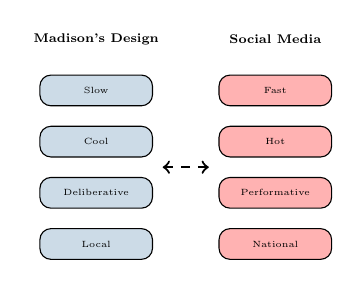
\begin{tikzpicture}[scale=0.65, transform shape,
    box/.style={draw, rounded corners, minimum width=2.2cm, minimum height=0.6cm, align=center, font=\tiny}]
  
  % Madison's Design
  \node[font=\scriptsize\bfseries] at (0,3.5) {Madison's Design};
  \node[box, fill=primaryblue!20] at (0,2.5) {Slow};
  \node[box, fill=primaryblue!20] at (0,1.5) {Cool};
  \node[box, fill=primaryblue!20] at (0,0.5) {Deliberative};
  \node[box, fill=primaryblue!20] at (0,-0.5) {Local};
  
  % Social Media
  \node[font=\scriptsize\bfseries] at (3.5,3.5) {Social Media};
  \node[box, fill=red!30] at (3.5,2.5) {Fast};
  \node[box, fill=red!30] at (3.5,1.5) {Hot};
  \node[box, fill=red!30] at (3.5,0.5) {Performative};
  \node[box, fill=red!30] at (3.5,-0.5) {National};
  
  \draw[<->, thick, dashed] (1.3,1) -- (2.2,1);
\end{tikzpicture}

\vspace{0.5em}
\begin{exampleblock}{\faQuoteLeft\hspace{0.2em}Haidt}
\tiny
\textit{``The tech companies that enhanced virality from 2009 to 2012 brought us deep into Madison's nightmare.''}
\end{exampleblock}
\end{column}
\end{columns}
\end{frame}

\begin{frame}{The Decline of Democratic Virtues}
\begin{table}
\centering
\scriptsize
\begin{tabular}{@{}p{2cm}p{3.8cm}p{5.5cm}@{}}
\toprule
\textbf{Virtue} & \textbf{What It Requires} & \textbf{How It's Being Undermined} \\
\midrule
\textbf{Civility} & Treating opponents as fellow citizens & Algorithms reward outrage; ``affective polarization'' \\
\textbf{Deliberation} & Listening, weighing evidence & Performative politics; echo chambers \\
\textbf{Trust} & Faith in institutions and shared facts & Disinformation; institutional failures \\
\textbf{Local Engagement} & Town halls, school boards & Nationalization of politics; decline of local news \\
\textbf{Tolerance} & Accepting reasonable disagreement & ``Cancel culture''; authoritarian populism \\
\textbf{Compromise} & Accepting partial victories & Primary voters reward purity \\
\bottomrule
\end{tabular}
\end{table}

\vspace{0.2em}
\begin{alertblock}{The Vicious Cycle}
As virtues decline $\rightarrow$ institutions work worse $\rightarrow$ trust falls further $\rightarrow$ virtues decline more
\end{alertblock}
\end{frame}

\begin{frame}{Policy Suggestions for Democratic Renewal}
\begin{columns}
\begin{column}{0.32\textwidth}
\begin{block}{Institutional}
\footnotesize
\begin{itemize}
  \item Open primaries, ranked-choice voting
  \item Nonpartisan redistricting
  \item Fund \textbf{local journalism}
\end{itemize}
\end{block}
\end{column}

\begin{column}{0.32\textwidth}
\begin{exampleblock}{Educational}
\footnotesize
\begin{itemize}
  \item Restore \textbf{humanities and civics}
  \item Teach ``narrative imagination''
  \item Support the arts
\end{itemize}
\end{exampleblock}
\end{column}

\begin{column}{0.32\textwidth}
\begin{alertblock}{Cultural/Civic}
\footnotesize
\begin{itemize}
  \item Revive \textbf{associations}
  \item Cross-partisan dialogue
  \item Local government
\end{itemize}
\end{alertblock}
\end{column}
\end{columns}

\vspace{0.3em}
\begin{exampleblock}{\faQuoteLeft\hspace{0.3em}Nussbaum}
\small
\textit{``Love is what gives respect for humanity its life, making it more than a shell.''}
\end{exampleblock}

\vspace{0.2em}
\discussion{Which suggestions would have the biggest impact? Which are most realistic?}
\end{frame}

% ====================
% PART IV: ARE WE GETTING WORSE? (Slides 32-37)
% ====================

\begin{frame}{The Case for Pessimism}
\begin{alertblock}{Evidence of Decline}
\begin{itemize}
  \item \textbf{Trust in institutions} at historic lows
  \item \textbf{Political polarization} increasing sharply
  \item \textbf{Teen mental health crisis}: Depression, anxiety rising since 2012
  \item Rise of \textbf{conspiracy theories}: QAnon, election denial
  \item ``\textbf{Structural stupidity}'': Dissent punished, bad ideas elevated
\end{itemize}
\end{alertblock}

\vspace{0.2em}
\begin{block}{The Tragedy of the Epistemic Commons}
\small
Just as individuals acting rationally can destroy shared environmental resources (tragedy of the commons), individuals making rational sharing decisions can \textbf{pollute our shared information environment}.
\end{block}

\vspace{0.2em}
\begin{exampleblock}{Regina Rini's Insight}
\small
Each person sharing something outrageous does little harm, but collectively we poison the well.
\end{exampleblock}
\end{frame}

\begin{frame}{Quote: Haidt on Structural Stupidity}
\begin{exampleblock}{\faQuoteLeft\hspace{0.5em}Jonathan Haidt, ``Why the Past 10 Years of American Life Have Been Uniquely Stupid'' (2022)}
\small
\textbf{Context:} Haidt argues that institutions become ``stupid'' when they punish internal dissent and reward conformity.

\vspace{0.5em}
\textit{``The most reliable cure for confirmation bias is \textbf{interaction with people who don't share your beliefs}. They confront you with counterevidence and counterargument... People who try to silence or intimidate their critics make themselves stupider, \textbf{almost as if they are shooting darts into their own brain}.''}
\end{exampleblock}

\vspace{0.5em}
\begin{block}{\faLightbulb\hspace{0.3em}The Paradox of Our Age}
We have \textbf{more information} than ever in human history, yet we seem to have \textbf{less shared understanding}. More data, less wisdom.
\end{block}
\end{frame}

\begin{frame}{The Case for Optimism}
\begin{block}{Evidence of Progress}
\begin{itemize}
  \item \textbf{\#MeToo movement}: Accountability for powerful abusers
  \item \textbf{Global coordination} on climate awareness
  \item Access to \textbf{education and information} unprecedented
  \item \textbf{Marginalized voices} can reach global audiences
  \item \textbf{Citizen journalism} exposes injustice
\end{itemize}
\end{block}

\vspace{0.3em}
\begin{exampleblock}{The ``Hidden Tribes'' Study}
\textbf{67\%} of Americans are the ``\textbf{exhausted majority}''---tired of polarization, willing to listen, seeking common ground. The vocal extremes are loud but \textit{small}.
\end{exampleblock}

\vspace{0.3em}
\begin{alertblock}{A Hopeful Possibility}
Perhaps the current dysfunction is a \textbf{transition phase}. We're still learning to adapt to new technologies---just as past generations adapted to print, radio, and television.
\end{alertblock}

\vspace{0.2em}
\discussion{Is the problem social media itself, or how we use it?}
\end{frame}

\begin{frame}{The Problem of Adaptive Preferences}
\begin{block}{Nussbaum's Concept: Adaptive Preferences}
People tend to \textbf{adjust their desires} to what seems achievable. If you've never known something better, you might not realize what you're missing.
\end{block}

\vspace{0.3em}
\begin{columns}
\begin{column}{0.48\textwidth}
\begin{alertblock}{The Worry}
Are we \textbf{adapting} to diminished forms of:
\begin{itemize}
  \item Attention?
  \item Friendship?
  \item Civic engagement?
  \item Shared reality?
\end{itemize}
...and calling it \textbf{normal}?
\end{alertblock}
\end{column}

\begin{column}{0.48\textwidth}
\begin{exampleblock}{The Counter-Worry}
Maybe we're just \textbf{nostalgic}:
\begin{itemize}
  \item Each generation adapts
  \item The past wasn't perfect either
  \item Change isn't always decline
  \item New goods emerge too
\end{itemize}
\end{exampleblock}
\end{column}
\end{columns}

\vspace{0.3em}
\begin{block}{\faLightbulb\hspace{0.3em}The Challenge}
How do we distinguish genuine decline from mere change? How do we know what we're missing if we've never had it?
\end{block}
\end{frame}

\begin{frame}{Borgmann's ``Hyperreality'' Revisited}
\begin{block}{Albert Borgmann (b. 1937)}
Philosopher of technology who warned in 1992 about ``\textbf{hyperreality}''---online environments offering ``stylized versions of ourselves'' competing with organic reality.
\end{block}

\vspace{0.2em}
\begin{exampleblock}{\faQuoteLeft\hspace{0.3em}Borgmann's Prescient Warning (1992)}
\small
\textit{``Social hyperreality has already begun to transform the social fabric... growing and thickening, \textbf{suffocating reality} and rendering humanity less mindful and intelligent.''}
\end{exampleblock}

\vspace{0.2em}
\begin{alertblock}{Long Dismissed as ``Moral Panic''---But Consider:}
\small
QAnon (millions believe elaborate fiction), election denial, COVID misinformation---have we lost a \textbf{shared reality}?
\end{alertblock}

\vspace{0.2em}
\discussion{When significant portions of the population believe demonstrably false things, have we entered ``hyperreality''?}
\end{frame}

\begin{frame}{What Would Aristotle Say?}
\begin{columns}
\begin{column}{0.48\textwidth}
\begin{alertblock}{Likely Concerns}
\begin{itemize}
  \item Virtue requires \textbf{practice}---do we practice patience, temperance, or their opposites?
  \item Virtue develops in \textbf{community}---are online ``communities'' real communities?
  \item Flourishing requires \textbf{leisure} for contemplation---does infinite scroll allow this?
  \item The mean requires \textbf{judgment}---do algorithms make judgment for us?
\end{itemize}
\end{alertblock}
\end{column}

\begin{column}{0.48\textwidth}
\begin{exampleblock}{Likely Appreciation}
\begin{itemize}
  \item Access to \textbf{knowledge}---Aristotle loved learning!
  \item Potential for \textbf{expanded friendship} networks
  \item Tools for \textbf{civic participation}
  \item New forms of \textbf{creative expression}
\end{itemize}
\end{exampleblock}

\vspace{0.5em}
\begin{block}{Probable Verdict}
A \textbf{cautious critic}---worried about defaults and incentive structures, but hopeful about potential if used wisely.
\end{block}
\end{column}
\end{columns}
\end{frame}

% ====================
% PART V: CRITICISMS AND CONCLUSION (Slides 38-41)
% ====================

\begin{frame}{Criticism 1: The Liberal Objection (Isaiah Berlin)}
\begin{block}{Isaiah Berlin (1909--1997)}
Political philosopher famous for distinguishing \textbf{negative liberty} (freedom \textit{from} interference) and \textbf{positive liberty} (freedom \textit{to} achieve self-realization).
\end{block}

\vspace{0.2em}
\begin{alertblock}{Berlin's Worry About Positive Liberty}
\small
``Positive liberty'' can become \textbf{tyrannical}: If we claim to know what human flourishing requires, we might force people to be ``free'' \textit{our way}. History is full of coercion ``for your own good.''
\end{alertblock}

\vspace{0.2em}
\begin{exampleblock}{Applied to Virtue Ethics}
\small
Who decides what counts as \textbf{virtue}? Isn't this just \textbf{paternalism}? What about people who \textit{choose} different visions of the good life?
\end{exampleblock}

\vspace{0.2em}
\discussion{Can we promote virtue without becoming paternalistic?}
\end{frame}

\begin{frame}{Criticism 2: The Nietzschean Objection}
\begin{block}{Friedrich Nietzsche (1844--1900)}
Radical critic of traditional morality who saw conventional virtues as expressions of ``\textbf{slave morality}.''
\end{block}

\vspace{0.2em}
\begin{alertblock}{The Objection}
\small
What we call ``virtues'' are often: humility, meekness, self-denial = the \textbf{weak consoling themselves}. True excellence requires going \textbf{beyond} conventional virtue. Great achievements often require what others call ``vices.''
\end{alertblock}

\vspace{0.2em}
\begin{exampleblock}{Modern Version}
\small
Many great artists, innovators, and leaders had \textbf{difficult personalities}. Steve Jobs was notoriously harsh. Would we want to ``cure'' them of their ``vices''?
\end{exampleblock}

\vspace{0.2em}
\discussion{Can you think of someone whose ``vices'' were essential to their achievements?}
\end{frame}

\begin{frame}{Defending Virtue Ethics}
\begin{columns}
\begin{column}{0.48\textwidth}
\begin{block}{Response to Berlin}
\small
\begin{itemize}
  \item Focus on \textbf{capabilities}, not coercion
  \item \textbf{Nussbaum}: Provide opportunities, let individuals choose
  \item \textbf{Enable} flourishing, don't define it rigidly
\end{itemize}
\end{block}
\end{column}

\begin{column}{0.48\textwidth}
\begin{block}{Response to Nietzsche}
\small
\begin{itemize}
  \item Aristotle includes \textbf{greatness of soul}---ambition is a virtue!
  \item \textbf{Practical wisdom} = knowing when rules don't apply
  \item Virtue ethics is more \textbf{flexible} than rules
\end{itemize}
\end{block}
\end{column}
\end{columns}

\vspace{0.3em}
\begin{alertblock}{The Stronger Claim}
In the digital age, we need virtue ethics \textit{more}, not less---because algorithms and platforms won't guide us toward flourishing on their own.
\end{alertblock}

\vspace{0.2em}
\begin{exampleblock}{\faLightbulb\hspace{0.3em}Key Insight}
We already shape character through education and culture. The question is \textit{how}, not \textit{whether}.
\end{exampleblock}
\end{frame}

\begin{frame}{Conclusion: The Stakes}
\begin{center}
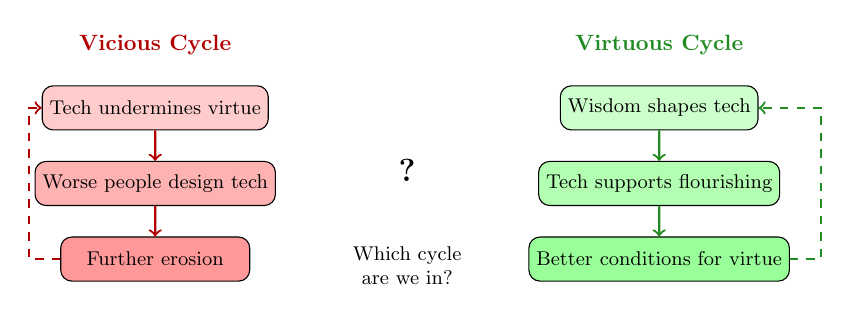
\begin{tikzpicture}[scale=0.8, transform shape,
    box/.style={draw, rounded corners, minimum width=3cm, minimum height=0.7cm, align=center, font=\small}]
  
  % Vicious Cycle (left)
  \node[font=\bfseries, text=red!70!black] at (-4,3) {Vicious Cycle};
  \node[box, fill=red!20] (v1) at (-4,2) {Tech undermines virtue};
  \node[box, fill=red!30] (v2) at (-4,0.8) {Worse people design tech};
  \node[box, fill=red!40] (v3) at (-4,-0.4) {Further erosion};
  \draw[->, thick, red!70!black] (v1) -- (v2);
  \draw[->, thick, red!70!black] (v2) -- (v3);
  \draw[->, thick, red!70!black, dashed] (v3.west) -- ++(-0.5,0) |- (v1.west);
  
  % Virtuous Cycle (right)
  \node[font=\bfseries, text=quotegreen] at (4,3) {Virtuous Cycle};
  \node[box, fill=green!20] (g1) at (4,2) {Wisdom shapes tech};
  \node[box, fill=green!30] (g2) at (4,0.8) {Tech supports flourishing};
  \node[box, fill=green!40] (g3) at (4,-0.4) {Better conditions for virtue};
  \draw[->, thick, quotegreen] (g1) -- (g2);
  \draw[->, thick, quotegreen] (g2) -- (g3);
  \draw[->, thick, quotegreen, dashed] (g3.east) -- ++(0.5,0) |- (g1.east);
  
  % Question in middle
  \node[font=\Large\bfseries] at (0,1) {?};
  \node[font=\small, text width=2.5cm, align=center] at (0,-0.5) {Which cycle\\are we in?};
\end{tikzpicture}
\end{center}

\vspace{0.3em}
\begin{block}{The Central Question}
\textbf{Will we shape technology, or will it shape us?}
\end{block}

\begin{exampleblock}{\faQuoteLeft\hspace{0.3em}Final Quote---Jonathan Haidt}
\small
\textit{``We cannot expect Congress and the tech companies to save us. \textbf{We must change ourselves and our communities}.''}
\end{exampleblock}

\end{frame}

\end{document}